\chapter{Work Experience} % Main chapter title

\label{Chapter2} % Change X to a consecutive number; for referencing this chapter elsewhere, use \ref{ChapterX}

\lhead{Chapter 2. \emph{Work Experience}} % Change X to a consecutive number; this is for the header on each page - perhaps a shortened title

I have had a total of six work placements since the start of my gap year.
Figure \ref{timeline} provides a timeline of the companies I have worked at.
The focus of this chapter will be on my placement at Sunamp, which was specifically done as part of my \textit{Industrial Project}.
After describing my experience at Sunamp, I will briefly describe my other work experiences.

\begin{figure}[htbp]
	\centering
	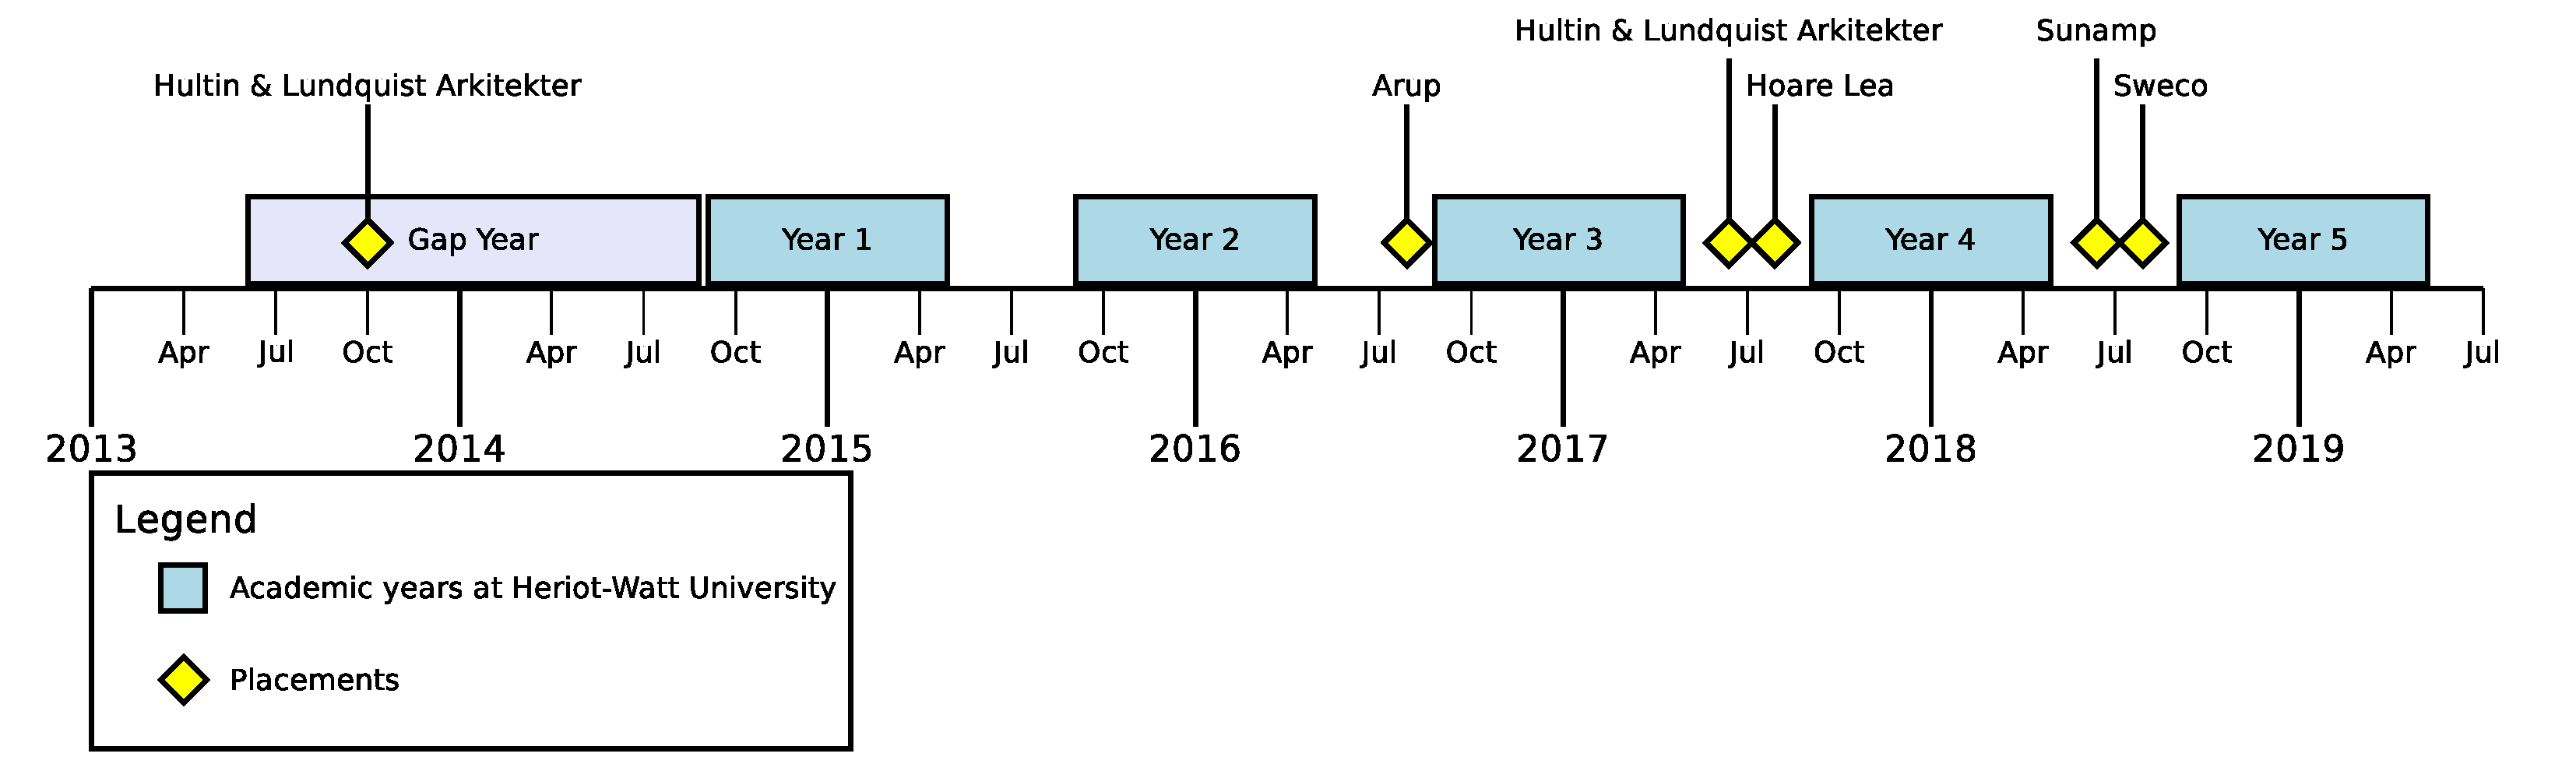
\includegraphics[width=\textwidth]{figures/IP-Timeline.eps}
	\rule{\textwidth}{0.5pt} % use line???
	\caption{Timeline of my work placements since my pre-university gap year.}
	\label{timeline}
\end{figure}


%----------------------------------------------------------------------------------------
%	SECTION 1
%----------------------------------------------------------------------------------------

\section{Sunamp, July - August 2018}

Sunamp is a newly established business that specialises in the research, production and sales of heat batteries that are based on phase change materials (PCMs).
The PCMs, developed and manufactured by Sunamp, are non-toxic, non-flammable, eco-friendly and patented in the UK and China, with patents pending in other countries \citep{SunampAutomotive}.
The PCMs operate at different temperatures, allowing the storage of heat (up to 100$^{\circ}$C and above) or coolth (less than 0$^{\circ}$C) (see Figure \ref{pcm_temp_range}).
Currently, the company's main markets are buildings, where their heat batteries can be used for the production of hot water and space heating, and automobiles, where their heat batteries can be used for the refrigeration of transported goods.

\begin{figure}[htbp]
	\centering
	\includegraphics[width=\textwidth]{figures/temperature-range-of-PCMs.jpg}
	\rule{\textwidth}{0.5pt} % use line???
	\caption{The temperature range of Sunamp's PCMs in degrees Celsius \citep{SunampAutomotive}.}
	\label{pcm_temp_range}
\end{figure}

Sunamp was founded by Andrew Bissell (CEO) and is based in Macmerry, East Lothian.
They have a small office building, which features a workshop and chemistry laboratory on the ground floor, and a factory across the road where they have additional test facilities but primarily do large-scale manufacturing and packaging of heat batteries.
Around 20 people work in the office and five in the factory.


%-----------------------------------
%	SUBSECTION 1
%-----------------------------------

\subsection{Description of work experience}

My placement at Sunamp started on Tuesday 3\textsuperscript{rd} July 2018 and ended on Friday 10\textsuperscript{th} August 2018.
I worked a total of 198 hours there across six weeks, averaging at about 6.8 hours of work per day (see log in Appendix ... \hl{blur out sensitive info before adding to appendix}).
\hl{My purpose/ job description ...}
My time at Sunamp can roughly be divided up into two \hl{areas/ aspects}: learning about Sunamp's work and development, and producing work for Sunamp.


\subsubsection{Learning about Sunamp}

The majority of my first week at Sunamp consisted of my familiarisation with the company and their products.
The week started with an induction from Susan Lang-Bissell (MD) where we went over my contract, office information, health and safety regulations (amongst other things) and I got a brief tour of the factory.
The induction was followed by an introduction from Joan Pisanek, the Business Development Manager, to UniQ (Sunamp's latest range of heat batteries for buildings) and some of Sunamp's projects.
I used the rest of the week to familiarise myself with and try to understand their products by consulting Joan's PowerPoint presentations and the UniQ manuals, working through Joan's Buchlyvie project (\hl{see Appendix ...}), and attempting a UniQ Product Training Exercise developed by Sandy.

Santokh Gataora, \hl{colloquially known as} Sandy, is Sunamp's Technical Director.
He has a vast experience in building services engineering and helped develop the UniQ product range.
He writes and continues to refine the UniQ manuals as he guides the company in the engineering and application aspects of their UniQ heat batteries in buildings.
When I joined the company, UniQ was a very recent development that the sales team was still learning about.
The week I arrived at Sunamp, Sandy had sent out an exercise for the sales team to complete for the following week's UniQ Product Training Workshop.
The exercise instructions and my attempted solution \hl{can be found in Appendix ...}.


%-----------------------------------
%	SUBSECTION 2
%-----------------------------------

\subsection{Analysis of/ Reflection on work experience}


%%%%%%%%%%%%%%%%%%%%%%%%%%%%%%%%%%%%%%%%%%%%%%%%%
\begin{comment}

\subsection{Application Process}

I learned about the opportunity of two paid placements with immediate start at Sunamp through David Campbell, the D11PJ course leader.
He had asked applicants for this placement to send him 100 words broadly describing their strengths and preferences, which he would then forward to Sunamp.
Hamish, a coursemate of mine, and I were both interested in this opportunity.
\hl{My hundred-word application went as follows:}

Strengths:
\begin{itemize}
	\item I am very familiar with the BIM process, having written a dissertation on collaboration with regards to BIM.
	\item I have work experience in mechanical and electrical consulting engineering.
	\item Organised, flexible, independent and cooperative.
\end{itemize}
Skills:
\begin{itemize}
	\item Advanced skills in Microsoft Office packages and Bluebeam Revu.
	\item Intermediate skills in LaTeX.
	\item Basic modelling skills in Revit, AutoCAD and IES-VE.
	\item Fluent in three languages (English, Swedish and French) with basic knowledge of Spanish.
\end{itemize}
Preferences/ interests:
\begin{itemize}
	\item Highly interested in learning about your application of Phase Change Materials in thermal storage batteries.
	\item Also interested in working with BIM and learning Bentley’s Hevacomp software packages.
\end{itemize}

After the applications, David introduced the two of us to Susan Lang-Bissell, the Managing Director (MD) of Sunamp, via email.
David asked us to liaise with Susan to arrange a meeting.
To do this, Hamish and I first established our availabilities in the upcoming days.
I then volunteered to liaise with Susan via email on our behalf to find a suitable date and time.

\hl{Try to be more reflective, and less descriptive.
Maybe record (vocally) the story, and then reflect on it out loud. THEN write about it.}

\end{comment}
